\chapter{Training a Convolutional Neural Network}
Once the network has been constructed the user needs to tune the hyperparameters in order to get the best loss and learning rate from their network in the shortest possible time. This is the most time consuming and frustrating part of the process as there are many different parts of the network that can be adjusted to produce different results. The three hyperparameters that need to be adjusted are as follows:
\begin{itemize}
    \item The number of filters in the convolutional layers
    \item The batch size
    \item The optimiser and the learning rate for said optimiser.
\end{itemize}
These will be discussed further in the following chapter. There are other hyperparameters that can be adjusted but considering the time and resources available this was not possible within the scope of this thesis. 
\par
At the end of this chapter there will be a brief discussion about the other hyperparamters that could have been adjusted that were not within the scope of this study. 
\section{Number of Filters}
The convolution depth determines the architecture of the neural network. The user has to decide what value to start with as this dictates how deep the output of the final convolutional layer will be. This variable was mentioned in Section \ref{sub.CNN}, where self.cr was the number of filters to be determined by the user. Most CNNs tend to use numbers that are a power of 2 for all stages of implementation, as we can see from Figure \ref{fig.filter_size} larger filters result in generally lower losses for our data. 
\begin{figure}[H]
\centering
\begin{subfigure}{0.45\textwidth}
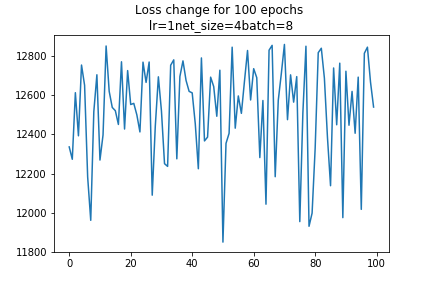
\includegraphics[width=\textwidth]{\dir/figs/learning_rate1net_size4batch8epochs100.png}
\caption{}
\label{fig.filter4l}
\end{subfigure}%
\hfill
\begin{subfigure}{0.45\textwidth}
\includegraphics[width=\textwidth]{\dir/figs/{learning_rate1net_size8batch8epochs100}.png}
\caption{}
\label{fig.filter8}
\end{subfigure}
\bigskip
\begin{subfigure}{0.45\textwidth}
\includegraphics[width=\textwidth]{\dir/figs/{learning_rate1net_size16batch8epochs100}.png}
\caption{}
\label{fig.filter16}
\end{subfigure}
\hfill
\begin{subfigure}{0.45\textwidth}
\includegraphics[width=\textwidth]{\dir/figs/{learning_rate1net_size32batch8epochs100}.png}
\caption{}
\label{fig.filter32}
\end{subfigure}
\caption[Effect of adjusting the filter size on Loss of network]{All four graphs show how adjusting the filter size effects the loss rate of the network after each epoch. (d) has a filter size of 32 and the loss here is generally smaller than in the other examples.}
\label{fig.filter_size}
\end{figure}
\section{Batch Size}
The batch size changes the size of the stack of data that is being fed into the neural network. A batch size of 1 will show a large fluctuation on the loss compared to a batch size the encompasses the whole dataset. A batch size that is the same size as the dataset should have small fluctuations in the loss unless the learning rate is too high. This is likely the case for the examples given in Figure \ref{fig.batch_size}
\begin{figure}[H]
\centering
\begin{subfigure}{0.45\textwidth}
\includegraphics[width=\textwidth]{\dir/figs/{learning_rate0.01net_size32batch8epochs100}.png}
\caption{}
\label{fig.br8l}
\end{subfigure}%
\hfill
\begin{subfigure}{0.45\textwidth}
\includegraphics[width=\textwidth]{\dir/figs/{learning_rate0.01net_size32batch16epochs100}.png}
\caption{}
\label{fig.br16}
\end{subfigure}
\bigskip
\begin{subfigure}{0.45\textwidth}
\includegraphics[width=\textwidth]{\dir/figs/{learning_rate0.01net_size32batch32epochs100}.png}
\caption{}
\label{fig.br32}
\end{subfigure}
\hfill
\begin{subfigure}{0.45\textwidth}
\includegraphics[width=\textwidth]{\dir/figs/{learning_rate0.01net_size32batch64epochs100}.png}
\caption{}
\label{fig.br64}
\end{subfigure}
\caption[Effect of adjusting the batch size on Loss of network]{All four graphs show how adjusting the batch size rate effects the loss rate of the network after each epoch. (d) The largest batch size shows consistently the lowest loss.}
\label{fig.batch_size}
\end{figure}
\section{Learning Rate and Optimizer}
The optimiser works to adjust the weights of the model before another training run is performed in order to decrease the loss of the network after each run. 
The standard optimiser for CNNs is Stochastic Gradient Descent, for this project a slight variation on this has been used, which is the ADAM optimiser. This works in a similar way but has some clever inbuilt variables that prevent the optimiser becoming stuck and the loss rate converging. 
  \begin{figure}[H]
\centering
\begin{subfigure}{0.45\textwidth}
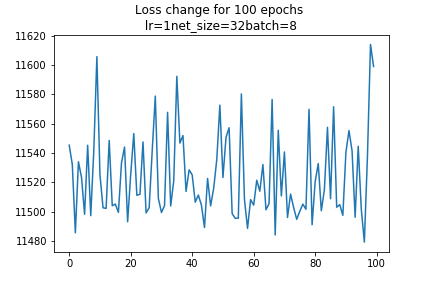
\includegraphics[width=\textwidth]{\dir/figs/learning_rate1net_size32batch8epochs100.png}
\caption{}
\label{fig.lr1l}
\end{subfigure}%
\hfill
\begin{subfigure}{0.45\textwidth}
\includegraphics[width=\textwidth]{\dir/figs/{learning_rate0.1net_size32batch8epochs100}.png}
\caption{}
\label{fig.lr0.1}
\end{subfigure}
\bigskip
\begin{subfigure}{0.45\textwidth}
\includegraphics[width=\textwidth]{\dir/figs/{learning_rate0.001net_size32batch8epochs100}.png}
\caption{}
\label{fig.lr0.001}
\end{subfigure}
\hfill
\begin{subfigure}{0.45\textwidth}
\includegraphics[width=\textwidth]{\dir/figs/{learning_rate0.0001net_size32batch8epochs100}.png}
\caption{}
\label{fig.lr0.0001}
\end{subfigure}
\caption[Effect of adjusting learning rate on Loss of network]{All four graphs show how adjusting the learning rate of the optimiser effects the loss rate of the network after each epoch. (b) returns the lowest loss, however there is a lot of fluctuation to the returned loss..}
\label{fig.learning_rate}
\end{figure}

\section{Testing the Network}